% Options for packages loaded elsewhere
\PassOptionsToPackage{unicode}{hyperref}
\PassOptionsToPackage{hyphens}{url}
\PassOptionsToPackage{dvipsnames,svgnames,x11names}{xcolor}
%
\documentclass[
  letterpaper,
  DIV=11,
  numbers=noendperiod]{scrartcl}

\usepackage{amsmath,amssymb}
\usepackage{iftex}
\ifPDFTeX
  \usepackage[T1]{fontenc}
  \usepackage[utf8]{inputenc}
  \usepackage{textcomp} % provide euro and other symbols
\else % if luatex or xetex
  \usepackage{unicode-math}
  \defaultfontfeatures{Scale=MatchLowercase}
  \defaultfontfeatures[\rmfamily]{Ligatures=TeX,Scale=1}
\fi
\usepackage{lmodern}
\ifPDFTeX\else  
    % xetex/luatex font selection
\fi
% Use upquote if available, for straight quotes in verbatim environments
\IfFileExists{upquote.sty}{\usepackage{upquote}}{}
\IfFileExists{microtype.sty}{% use microtype if available
  \usepackage[]{microtype}
  \UseMicrotypeSet[protrusion]{basicmath} % disable protrusion for tt fonts
}{}
\makeatletter
\@ifundefined{KOMAClassName}{% if non-KOMA class
  \IfFileExists{parskip.sty}{%
    \usepackage{parskip}
  }{% else
    \setlength{\parindent}{0pt}
    \setlength{\parskip}{6pt plus 2pt minus 1pt}}
}{% if KOMA class
  \KOMAoptions{parskip=half}}
\makeatother
\usepackage{xcolor}
\usepackage{svg}
\setlength{\emergencystretch}{3em} % prevent overfull lines
\setcounter{secnumdepth}{-\maxdimen} % remove section numbering
% Make \paragraph and \subparagraph free-standing
\makeatletter
\ifx\paragraph\undefined\else
  \let\oldparagraph\paragraph
  \renewcommand{\paragraph}{
    \@ifstar
      \xxxParagraphStar
      \xxxParagraphNoStar
  }
  \newcommand{\xxxParagraphStar}[1]{\oldparagraph*{#1}\mbox{}}
  \newcommand{\xxxParagraphNoStar}[1]{\oldparagraph{#1}\mbox{}}
\fi
\ifx\subparagraph\undefined\else
  \let\oldsubparagraph\subparagraph
  \renewcommand{\subparagraph}{
    \@ifstar
      \xxxSubParagraphStar
      \xxxSubParagraphNoStar
  }
  \newcommand{\xxxSubParagraphStar}[1]{\oldsubparagraph*{#1}\mbox{}}
  \newcommand{\xxxSubParagraphNoStar}[1]{\oldsubparagraph{#1}\mbox{}}
\fi
\makeatother


\providecommand{\tightlist}{%
  \setlength{\itemsep}{0pt}\setlength{\parskip}{0pt}}\usepackage{longtable,booktabs,array}
\usepackage{calc} % for calculating minipage widths
% Correct order of tables after \paragraph or \subparagraph
\usepackage{etoolbox}
\makeatletter
\patchcmd\longtable{\par}{\if@noskipsec\mbox{}\fi\par}{}{}
\makeatother
% Allow footnotes in longtable head/foot
\IfFileExists{footnotehyper.sty}{\usepackage{footnotehyper}}{\usepackage{footnote}}
\makesavenoteenv{longtable}
\usepackage{graphicx}
\makeatletter
\def\maxwidth{\ifdim\Gin@nat@width>\linewidth\linewidth\else\Gin@nat@width\fi}
\def\maxheight{\ifdim\Gin@nat@height>\textheight\textheight\else\Gin@nat@height\fi}
\makeatother
% Scale images if necessary, so that they will not overflow the page
% margins by default, and it is still possible to overwrite the defaults
% using explicit options in \includegraphics[width, height, ...]{}
\setkeys{Gin}{width=\maxwidth,height=\maxheight,keepaspectratio}
% Set default figure placement to htbp
\makeatletter
\def\fps@figure{htbp}
\makeatother

\KOMAoption{captions}{tableheading}
\makeatletter
\@ifpackageloaded{caption}{}{\usepackage{caption}}
\AtBeginDocument{%
\ifdefined\contentsname
  \renewcommand*\contentsname{Table of contents}
\else
  \newcommand\contentsname{Table of contents}
\fi
\ifdefined\listfigurename
  \renewcommand*\listfigurename{List of Figures}
\else
  \newcommand\listfigurename{List of Figures}
\fi
\ifdefined\listtablename
  \renewcommand*\listtablename{List of Tables}
\else
  \newcommand\listtablename{List of Tables}
\fi
\ifdefined\figurename
  \renewcommand*\figurename{Figure}
\else
  \newcommand\figurename{Figure}
\fi
\ifdefined\tablename
  \renewcommand*\tablename{Table}
\else
  \newcommand\tablename{Table}
\fi
}
\@ifpackageloaded{float}{}{\usepackage{float}}
\floatstyle{ruled}
\@ifundefined{c@chapter}{\newfloat{codelisting}{h}{lop}}{\newfloat{codelisting}{h}{lop}[chapter]}
\floatname{codelisting}{Listing}
\newcommand*\listoflistings{\listof{codelisting}{List of Listings}}
\makeatother
\makeatletter
\makeatother
\makeatletter
\@ifpackageloaded{caption}{}{\usepackage{caption}}
\@ifpackageloaded{subcaption}{}{\usepackage{subcaption}}
\makeatother

\ifLuaTeX
  \usepackage{selnolig}  % disable illegal ligatures
\fi
\usepackage{bookmark}

\IfFileExists{xurl.sty}{\usepackage{xurl}}{} % add URL line breaks if available
\urlstyle{same} % disable monospaced font for URLs
\hypersetup{
  pdftitle={Kobotoolbox Tutorial},
  pdfauthor={Felipe Valdez felipe.valdez@temple.edu},
  colorlinks=true,
  linkcolor={blue},
  filecolor={Maroon},
  citecolor={Blue},
  urlcolor={Blue},
  pdfcreator={LaTeX via pandoc}}


\title{Kobotoolbox Tutorial}
\author{Felipe Valdez felipe.valdez@temple.edu}
\date{}

\begin{document}
\maketitle

\renewcommand*\contentsname{Table of contents}
{
\hypersetup{linkcolor=}
\setcounter{tocdepth}{3}
\tableofcontents
}

\subsection{Introduction}\label{introduction}

This tutorial will guide you through the first steps for using
KoboToolbox, from creating an account, generating a form with different
types of questions, collecting data online and offline, exporting and
visualizing data.

\subsection{What is Kobotoolbox?}\label{what-is-kobotoolbox}

\href{https://www.kobotoolbox.org/about-us/software/}{KoboToolbox} is an
open source platform for the collection, management, and visualization
of data. As the most widely used primary data collection tool in the
nonprofit sector, it is the tool of choice for over 14,000 social impact
organizations worldwide.

\includesvg{kobotoolbox_tutorial_files/mediabag/kobotoolbox_logo_def.svg}
\textbf{Kobotoolbox features}

\begin{itemize}
\tightlist
\item
  Build questionnaires in the web or using XLSForm
\item
  Translate questionnaires into multiple languages
\item
  Create a questions library
\item
  Collect data offline or online in multiple devices (mobile phones,
  tablets, laptops)
\item
  Visualize data in maps and reports
\item
  Download data in multiple formats (XLS, CSV, KML, ZIP, GeoJSON)
\item
  Share and collaborate on projects
\end{itemize}

\subsection{Getting started in
KoboToolbox}\label{getting-started-in-kobotoolbox}

\textbf{1. Create an account}

\begin{enumerate}
\def\labelenumi{\arabic{enumi}.}
\item
  Go to \url{https://www.kobotoolbox.org/sign-up/}
\item
  Select `Global KoboToolbox Server'
\item
  Enter the required information in the form and click on create
  account.
\end{enumerate}

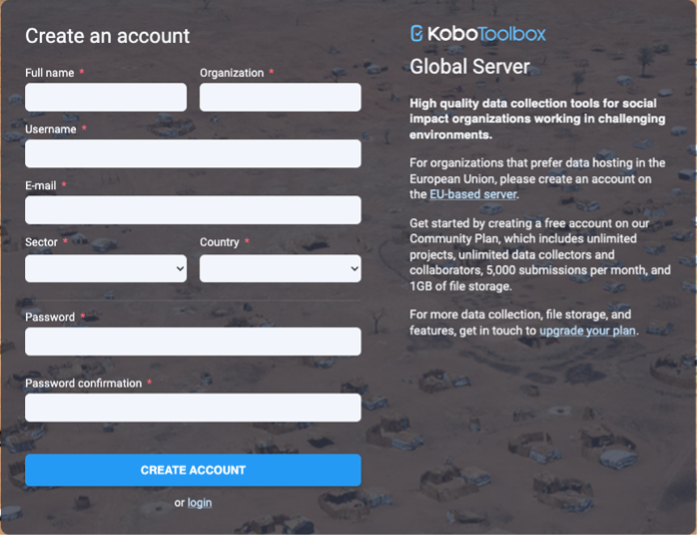
\includegraphics{kobotoolbox_tutorial_files/img/img1.png}

\textbf{2. Login to KoboToolbox}

\begin{enumerate}
\def\labelenumi{\arabic{enumi}.}
\item
  Go to \url{https://kf.kobotoolbox.org/account/login}
\item
  Enter your username and password
\end{enumerate}

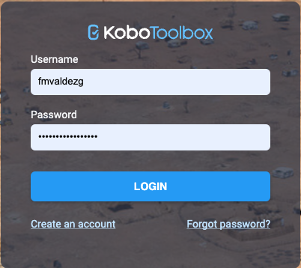
\includegraphics{kobotoolbox_tutorial_files/img/img2.png}

\textbf{My Projects Dashboard}

In the My Projects View you will find all your projects listed. You can
see on the left side a list of the Status of your projects just below
the `New' button. On the upper right you will find three option to apply
to your projects: archive, share or delete.

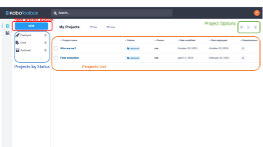
\includegraphics{kobotoolbox_tutorial_files/img/img3.png}

\subsection{Creating a new
questionnaire}\label{creating-a-new-questionnaire}

\begin{enumerate}
\def\labelenumi{\arabic{enumi}.}
\item
  Login to your account (see step 2 on
  \href{https://6f55d0be68b34246b8b812a68d153338.app.posit.cloud/p/b6def2a0/\#getting-started-in-kobotoolbox}{previous
  section})
\item
  On the \emph{My Projects} view, click on \texttt{New}
  
\includegraphics{kobotoolbox_tutorial_files/img/img4.png}
\item
  Select the option \texttt{Build\ from\ scratch}
\end{enumerate}

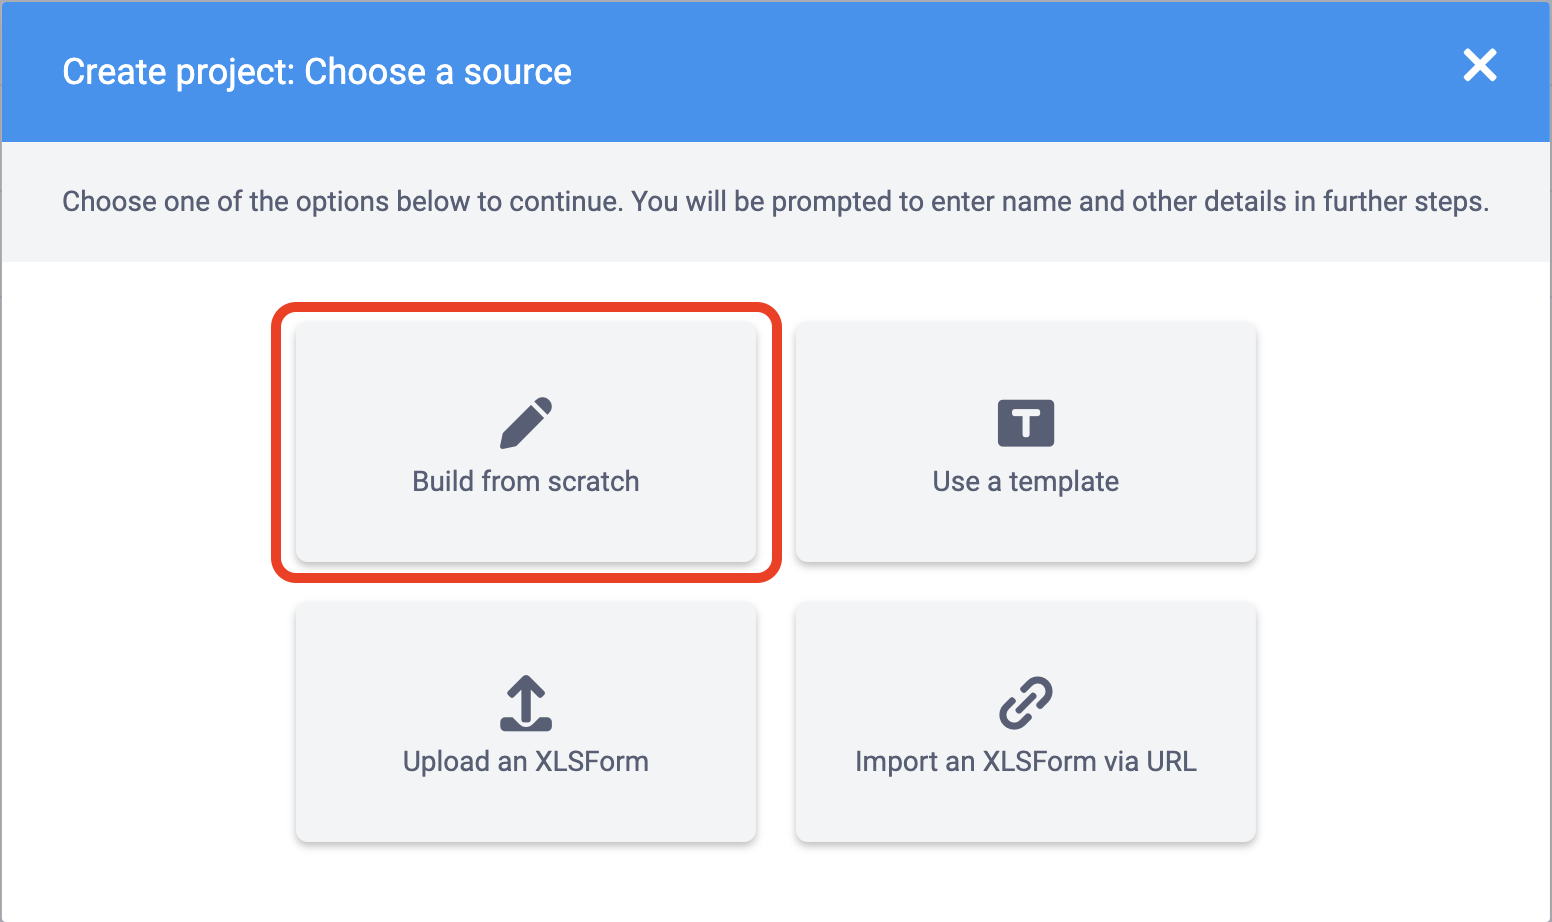
\includegraphics{kobotoolbox_tutorial_files/img/img5.png}

\begin{enumerate}
\def\labelenumi{\arabic{enumi}.}
\setcounter{enumi}{3}
\tightlist
\item
  Enter a title for your project, along with a sector and a country.
  Then click on \texttt{Create\ Project}.
\end{enumerate}

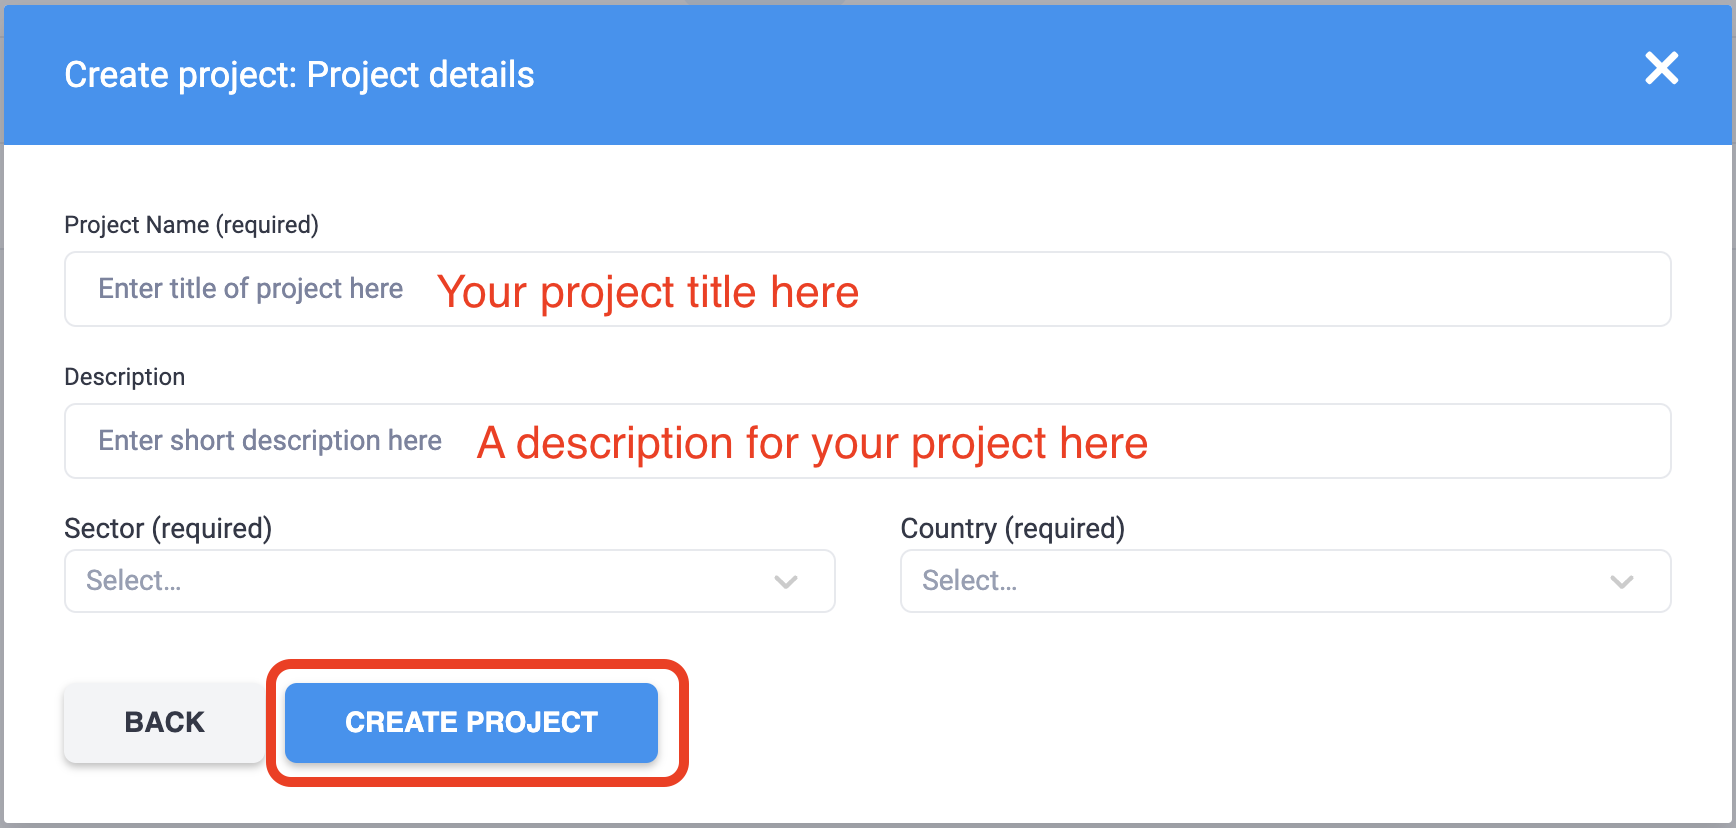
\includegraphics{kobotoolbox_tutorial_files/img/img6.png}

\begin{enumerate}
\def\labelenumi{\arabic{enumi}.}
\setcounter{enumi}{4}
\item
  Start adding new questions by clicking on the
  
\includegraphics{kobotoolbox_tutorial_files/img/img6_1.png} button and
  then \texttt{Add\ a\ question}.
\item
  We are going to add a \texttt{Select\ One} type question by clicking
  over the first option.
  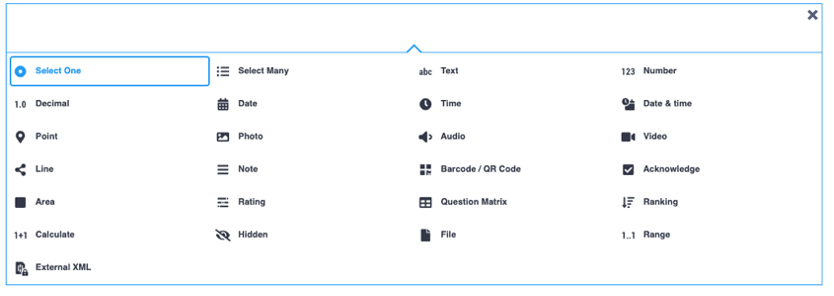
\includegraphics{kobotoolbox_tutorial_files/img/img7.png}
\item
  In the new question, you will have a space to add the question prompt,
  a hint on how to respond and a list of options to respond the
  question. 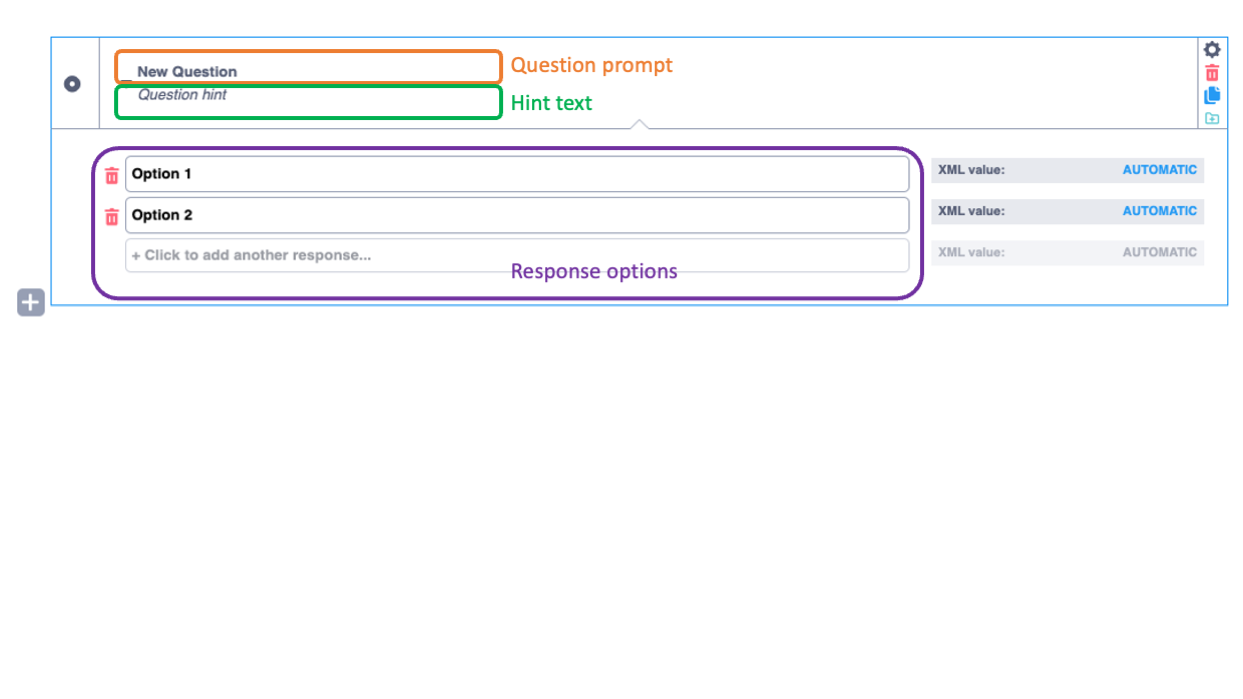
\includegraphics{kobotoolbox_tutorial_files/img/img8.png}
\item
  Once you are done creating questions, you can click on
  
\includegraphics{kobotoolbox_tutorial_files/img/img9.png} button
  located on the upper right corner of the screen.
\item
  Click on the \texttt{Retunr\ to\ list}
  
\includegraphics{kobotoolbox_tutorial_files/img/img10.png} button
  located on the upper left corner to go back to the dashboard
\end{enumerate}

\subsection{Deploying and sharing a
questionnaire}\label{deploying-and-sharing-a-questionnaire}

\begin{enumerate}
\def\labelenumi{\arabic{enumi}.}
\tightlist
\item
  Preview your questionnaire:
\end{enumerate}

Once you are done creating the questionnaire, you might like to preview
it. To do so, click on the name of your project on the list in the
dashborad.

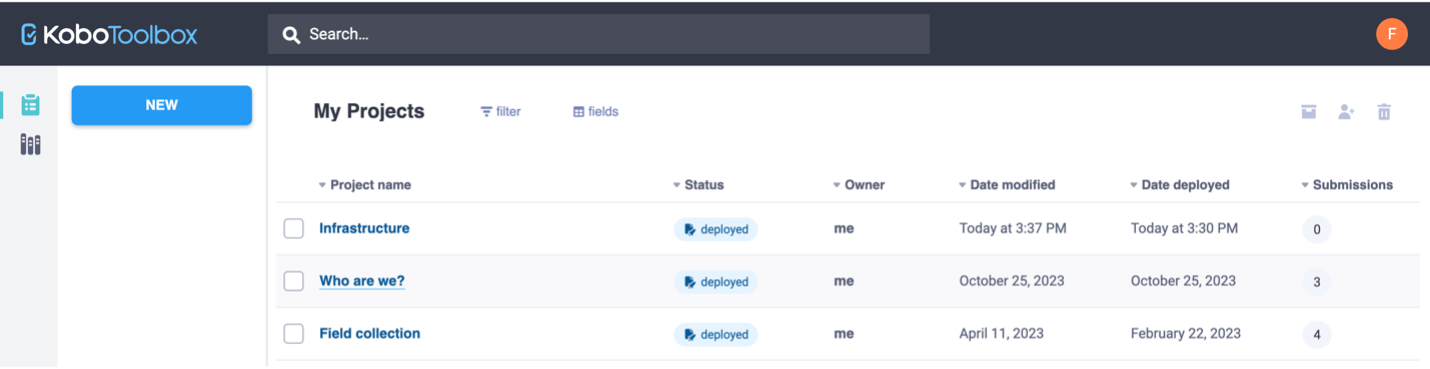
\includegraphics{kobotoolbox_tutorial_files/img/img11.png}

You will see a summary of the project, displaying the description, the
project status, number of questions, the owner, last time modified and
deployed. Also, on the bottom of the page you will see a chart and
statistics of the submissions.

To preview your questionnaire, click on \texttt{Preview\ form} on the
Quick Links menu on the right of the screen.

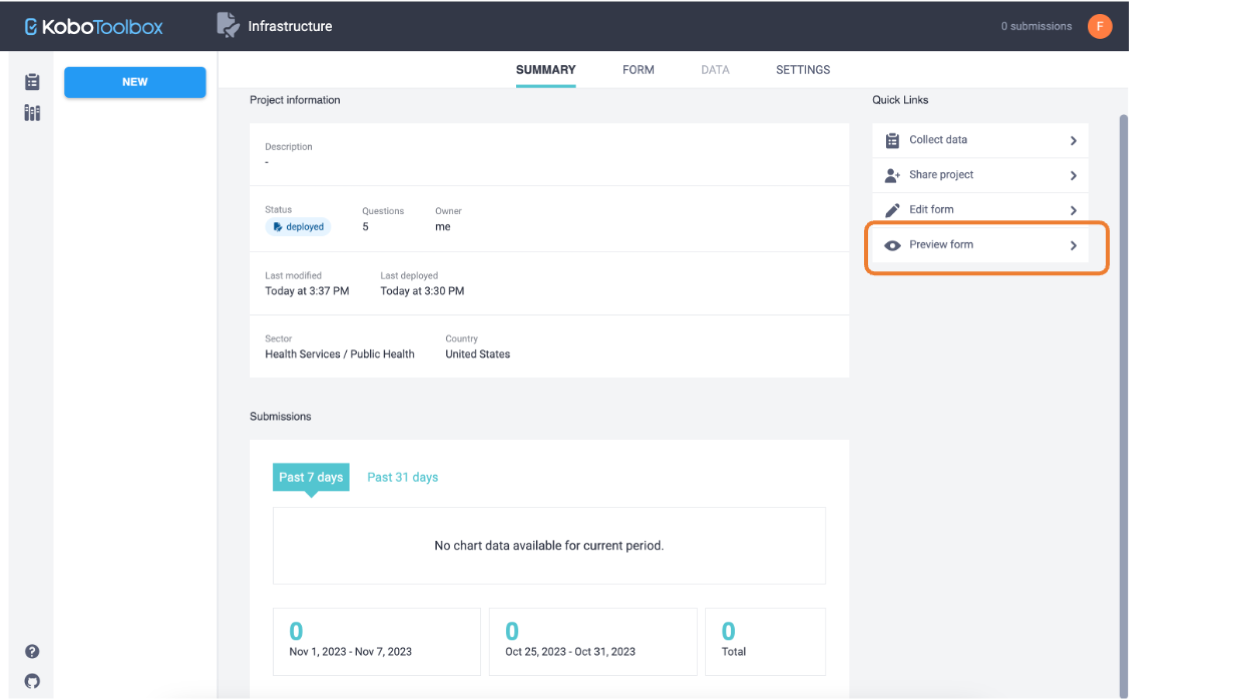
\includegraphics{kobotoolbox_tutorial_files/img/img12.png}

A temporary popup windows will show a complete functional version of the
form. You can fill up the questions, but the responses will not be
loaded to your project.

\begin{enumerate}
\def\labelenumi{\arabic{enumi}.}
\setcounter{enumi}{1}
\tightlist
\item
  Deploy the questionnaire
\end{enumerate}

Deploying your form is needed to make it available to the public, or to
those who will be filling the form in the field.

To deploy the form, click on \texttt{FORM} menu on the top of the
screen, next to \texttt{SUMMARY}. Then, click on the \texttt{DEPLOY} (or
\texttt{REDEPLOY} if you made changes to the form) button.

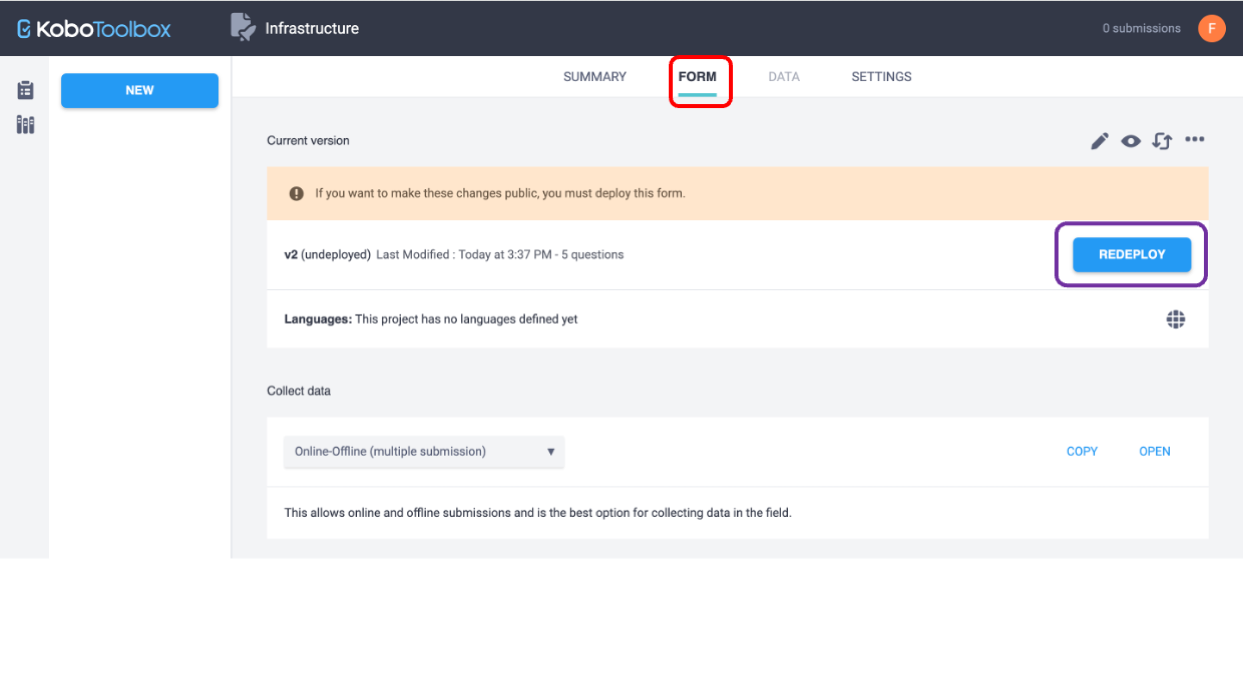
\includegraphics{kobotoolbox_tutorial_files/img/img13.png}

Remember to redeploy your form each time you made changes to the
questions in order to see them in the form you are sharing.

\begin{enumerate}
\def\labelenumi{\arabic{enumi}.}
\setcounter{enumi}{2}
\tightlist
\item
  Preparing the for before data collection
\end{enumerate}

Before starting to collect data, you will want to set up the mode of
collection. In the same window \texttt{FORM}, under the section
\texttt{Collect\ data} you will see a drop-down menu with multiple
options. Select the one that best adapts to the type of collection you
will be doing. In this case, we will set it on
\texttt{Online-Offline\ (multiple\ submissions)} as we want to collect
data without being connected to the internet.

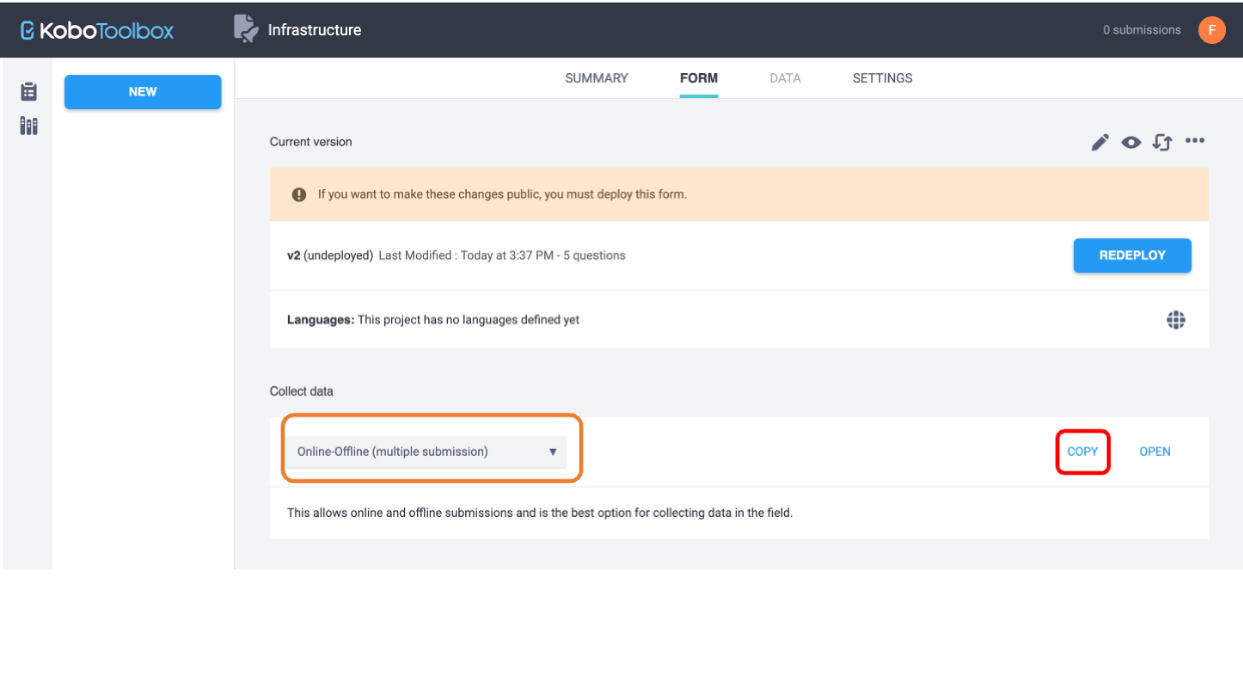
\includegraphics{kobotoolbox_tutorial_files/img/img14.png}

Now, to start collecting the data you can simply click on the
\texttt{COPY} button to copy the URL of your form. You can share this
url with the people that will be adding entries to the form.

Or you can click on \texttt{OPEN} to open the form from the browser on
the device you are using.

\subsection{Collecting data on a mobile
device}\label{collecting-data-on-a-mobile-device}

\begin{enumerate}
\def\labelenumi{\arabic{enumi}.}
\tightlist
\item
  Once you open the URL of the form, if the form includes a location
  question, you will see a message asking to provide access to location
  services. Be sure to \texttt{allow\ access} if you want to be able to
  use the location of your phone in the form.
\end{enumerate}

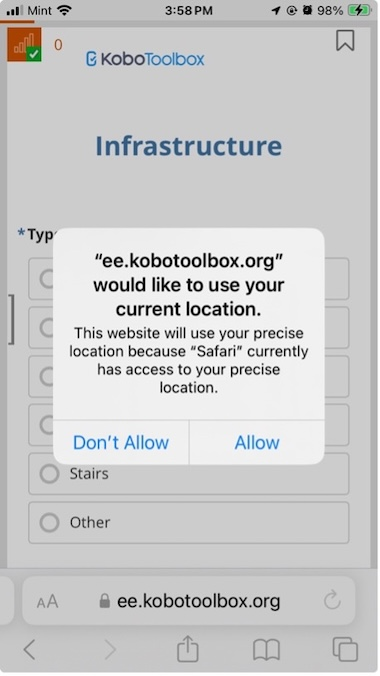
\includegraphics{kobotoolbox_tutorial_files/img/img15.jpg}

\begin{enumerate}
\def\labelenumi{\arabic{enumi}.}
\setcounter{enumi}{1}
\tightlist
\item
  Fill out the questions as needed.
\end{enumerate}

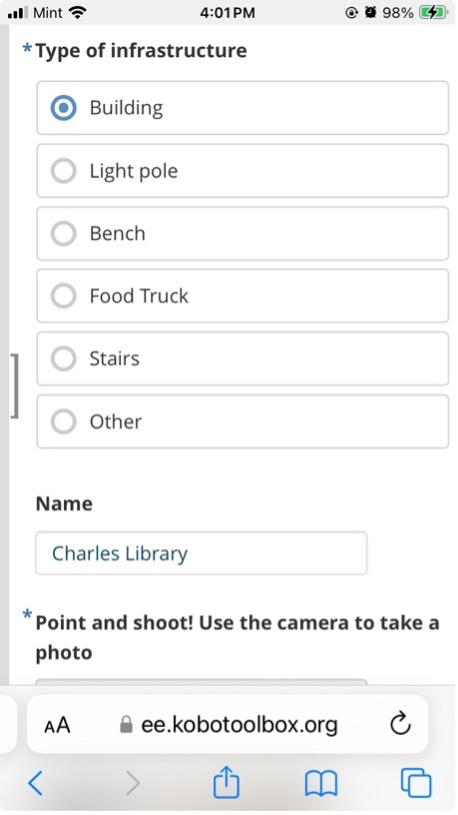
\includegraphics{kobotoolbox_tutorial_files/img/img16.jpg}

\begin{enumerate}
\def\labelenumi{\arabic{enumi}.}
\setcounter{enumi}{2}
\tightlist
\item
  If there is a location question on the form. Click on the record the
  current location icon.
  
\includegraphics{kobotoolbox_tutorial_files/img/img17_1.png}
\end{enumerate}

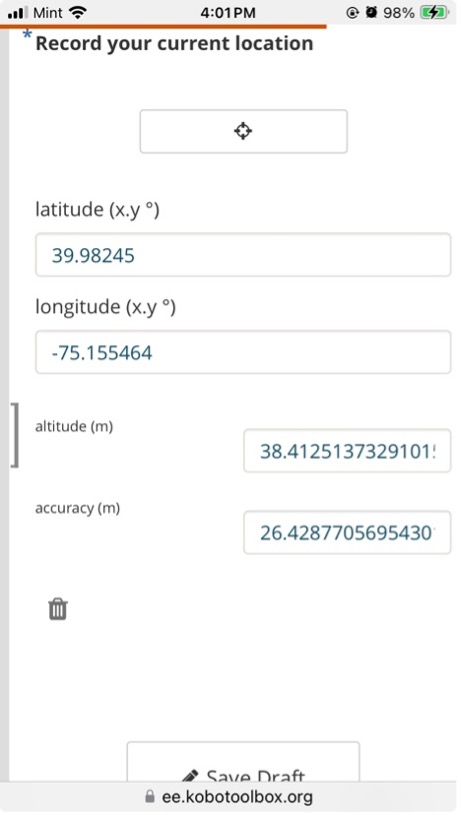
\includegraphics{kobotoolbox_tutorial_files/img/img17.jpg}

\begin{enumerate}
\def\labelenumi{\arabic{enumi}.}
\setcounter{enumi}{3}
\tightlist
\item
  Once you are done filling the questions, and you get to the bottom of
  the form, click on \texttt{Submit\ form}.
\end{enumerate}

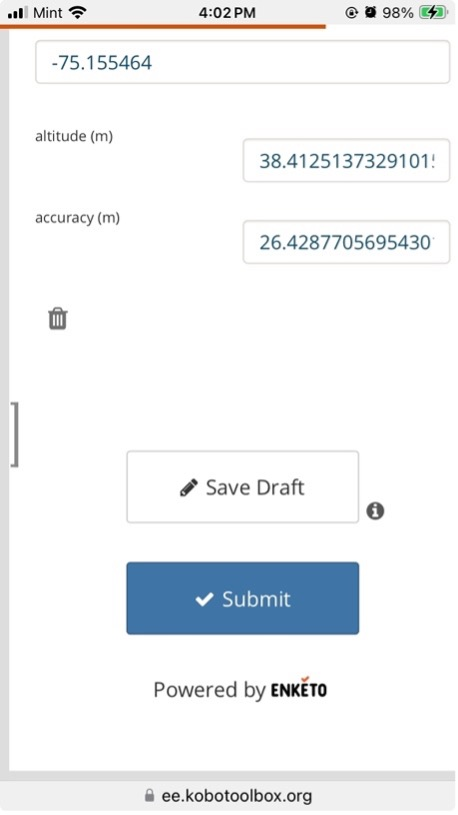
\includegraphics{kobotoolbox_tutorial_files/img/img18.jpg}

\subsection{Collecting data offline}\label{collecting-data-offline}

\textbf{Before} going to the field or while you are \textbf{still
online}, be sure to follow these steps:

\begin{enumerate}
\def\labelenumi{\arabic{enumi}.}
\item
  Open the form using the URL when you are still online.
\item
  To bookmark the form, if you are using an iPhone, click on the
  \texttt{Share} option
  
\includegraphics{kobotoolbox_tutorial_files/img/img20.png}
\item
  Click on \texttt{Add\ to\ home\ screen}.
\end{enumerate}

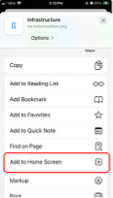
\includegraphics{kobotoolbox_tutorial_files/img/img21.png}

\begin{enumerate}
\def\labelenumi{\arabic{enumi}.}
\setcounter{enumi}{3}
\tightlist
\item
  You will see an icon created on your home screen with the name of your
  form 
\includegraphics{kobotoolbox_tutorial_files/img/img22.jpg}
\end{enumerate}

Warning! Do not clear you internet browser history if you are collecting
data offline.

Well done! Always use the homescreen shortcut you just created to open
the form.

\begin{enumerate}
\def\labelenumi{\arabic{enumi}.}
\setcounter{enumi}{4}
\tightlist
\item
\end{enumerate}




\end{document}
